\subsection{Example: Initial Condition and Rate of Something Decaying}\label{ex:decay-set-sample-accuracy}

\begin{figure}[h]
\begin{minipage}{.4\textwidth}
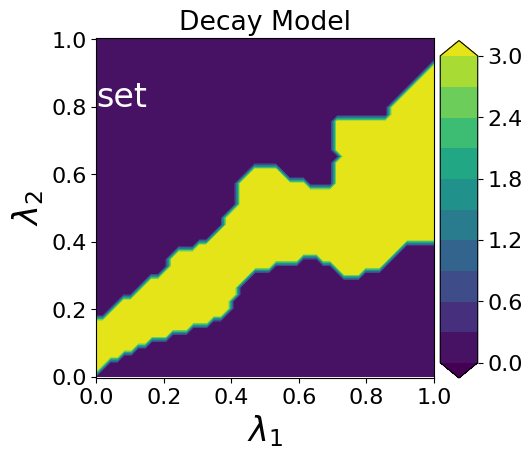
\includegraphics[width=\linewidth]{examples/fig_decay_q1/DecayModel--set_N50_em.png}
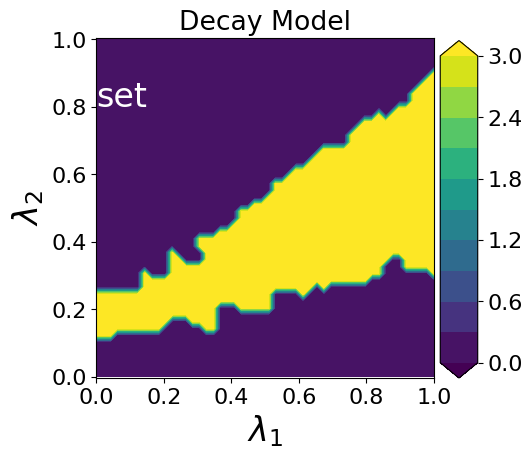
\includegraphics[width=\linewidth]{examples/fig_decay_q1/DecayModel--set_N500_em.png}

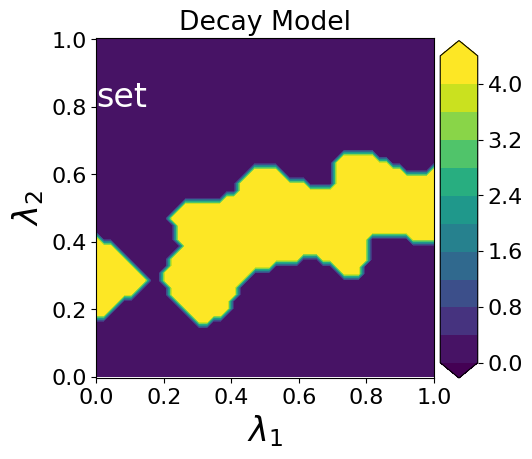
\includegraphics[width=\linewidth]{examples/fig_decay_q2/DecayModel--set_N50_em.png}
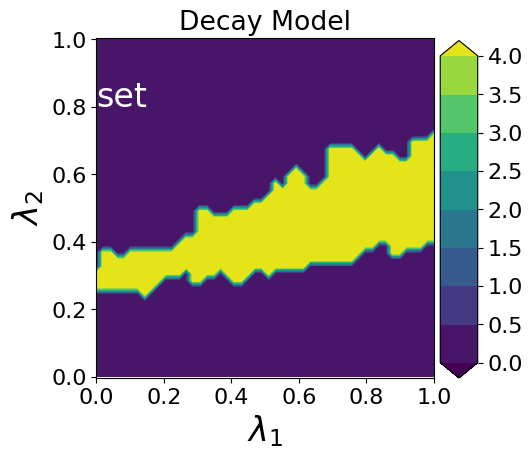
\includegraphics[width=\linewidth]{examples/fig_decay_q2/DecayModel--set_N500_em.png}
\end{minipage}
\begin{minipage}{.4\textwidth}
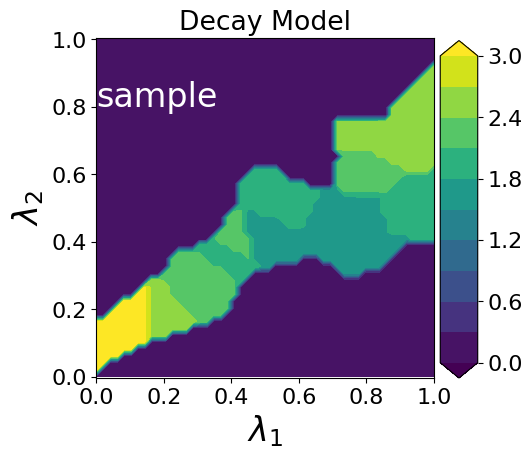
\includegraphics[width=\linewidth]{examples/fig_decay_q1/DecayModel--sample_N50_mc.png}
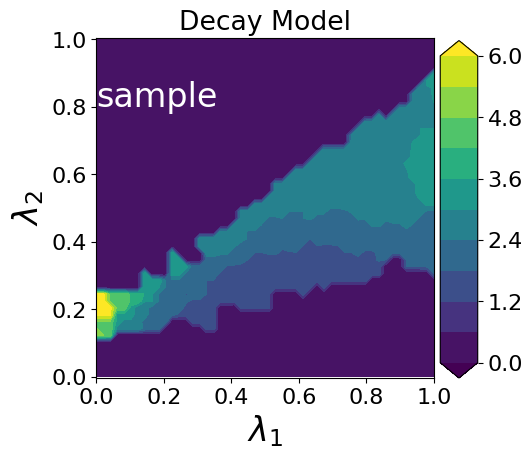
\includegraphics[width=\linewidth]{examples/fig_decay_q1/DecayModel--sample_N500_mc.png}

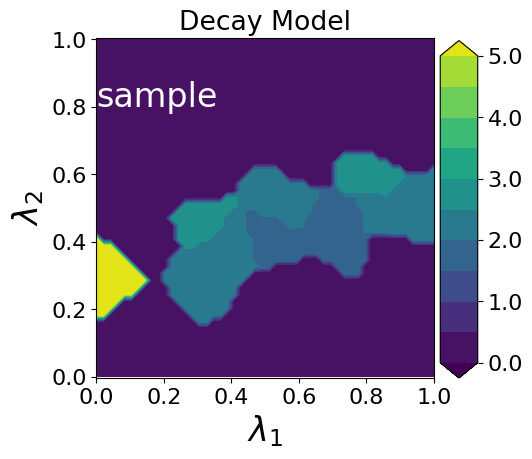
\includegraphics[width=\linewidth]{examples/fig_decay_q2/DecayModel--sample_N50_mc.png}
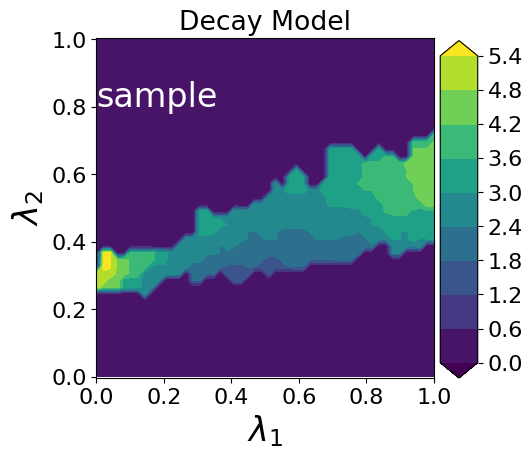
\includegraphics[width=\linewidth]{examples/fig_decay_q2/DecayModel--sample_N500_mc.png}
\end{minipage}

\caption{The inverse image of the reference measure for $\qoiA$ (top half) and $\qoiB$ (bottom half). }
\label{fig:decay-convergence}
\end{figure}

With these nonlinear cases, we find that taking an ``on average'' approach is inefficient, as there can be dramatic differences in the geometric properties of the inverse images in the parameter space depending on the location.
These results motivate further study into utilizing different QoI maps (perhaps some of those other four combinations available to us in this example) depending on where the samples came from in the parameter space.
In general, we saw in this example that given that two maps invert into sets of similar size on average, using the one with lower skewness results in less samples required to accurately approximate the inverse image.
The maps we used had average skewnesses that differed by 0.5 (instead of by 1), and the trend from the linear examples still held in significant portions of the parameter space.
